\chapter*{Summary}
\chaptermark{}
\addcontentsline{toc}{chapter}{Summary - Samenvatting}

{\Large\bf
  The Weak Phase \phis and Penguin Topologies.
}
\vspace*{0.05\textwidth}

Within the domain of modern pysics there exists a particular field of research
that attempts to answer a fundamental question about the natural world. This
question follows intuitivelly when observing the natural world and it troubled
philospphers since the ancient times. These philosophers attempted to understand
which are the fundamental blocks that build the world around them. Remarkably
enough after more that 2000 years since Democitus, who is commonly accepted as
the first person that introduced the idea of idivisible blocks of nature named
atoms (or \textgreek{άτομα} in Greek), contemprary scientists still have not found a definite
answer on the fundamental blocks of nature. So far, it seems that the observable
universe consists of a handful of elementary particles, which are clasified in two
distinct categories, namely {\it gauge bosons}, responsible for mediating all the
known fundamental forces of nature (with the exception of gravity) and {\it fermions}
which are the constituents of matter. There are 5 gauge bosons and 12 fermions.
Fermions can be divided further into {\it quarks}, which constitute composite
particles like the proton. A typical {\it lepton} is the electron which orbits
the nucleus of all atoms.

\subsubsection{Particle Physics and The Standard Model}
The state of the art mathematical framework necessary to describe the interactions between the
fermions is called the \textit{Standard Model} of Particle Physics \cite{sm-glashow,sm-weinberg,sm-salam}.
Describing an interaction in this context means being able to predict the probability for a certain
outcome in a (fundamental) particle colision. Given the fact that energy and mass can convert
from one to the other, the type of the initial and final particles is not the same. For example,
two initial quarks can colide, or more precicely annihilate, and produce an electron-positron pair.
This is counter intuitive compared to the clasical, non-quantum, description of particle collisions,
where the atomic structure of particles does not change. Thus, the established predictive power of
the Standard Model is an important achievement of particle physicists. Furthermore, the recently
discovered Higgs boson \cite{higgs-cms,higgs-atlas}, which plays a special role in explaining how
particles acquire mass, makes the Standard Model robust.

Despite the its sucess in describing the outcome of particle interactions, there are certain
established phenomena and observations that Standard Model does not account for.
Perhaps the most striking one is the absence of any description about the most familiar,
yet the weakest, force of nature, meaning gravity. Or perhaps the observed matter-antimatter
asymmetry in the universe \cite{more-cpv-huet,more-cpv-gavela_I,more-cpv-gavela_II}.
Note that antimatter is a well understood state of matter that has its quantum numbers sign,
such as electric charge, flipped with respect to matter. The above phenomena are a few
examples that reveal the incompletness of the model. Thus the scientific method compels
scientists to continue testing Standard Model predictions and look for ways to improve it.
Any significant diviation from these predictions could hint the presence of
{\it New Physics} beyond the established model.

\subsubsection{\CP Violation}
According to the dominant consensus regarding the matter-antimatter balance in the
universe, it is believed that during the big bang matter and antimatter existed at
equal proportions. This idea invites the notion of the so called Charge-Parity (\CP)
symmetry between matter and antimatter. Perfect \CP symmetry when it comes to particle
interactions imply that nature interacts both with matter and antimatter at the same rate.
However, at current time the observable universe seems to be almost entirely populated by
matter. Given this observation, the origin of this violation of the \CP symmetry follows
as a natural question.

The established idea that nature favours processes where the final particles are matter
and not antimatter particles is indeed captured by the Standard Model. It addition, it
is intreasting to point out that the origin of \CP violation is very closely releated
to the mechanism that the fermions aquire mass, which is the Higgs boson. However,
despite the fact that the Standard Model allows for the presence of \CP violation,
it cannot account for the observed ammount of matter-antimatter asymmetry.
Hence, other sources of \CP violation beyond the Standard Model have to be active.

The ammount of \CP violation is typically quantified by several parameters for which
the predicted by the Standard Model values have to be compared against the experimentally
measured values. Potential descrepancy between the prediction and the measured value
provide hints for the presence of New Physics. It is intreasting to point out that all these paramters have to yield
a consistent picture with each other. This offers a powerful discrimination between alternative models that might
modify Standard Model predictions. In other words these alternative models have to
modify all the \CP violating parameters in a consistent way.


\subsubsection{The Weak Phase \phis}
Violation of the \CP symmetry in particle physics typicaly manifests itself when comparing
the rate, or probability, of two particle decays. The two decays are releated by a \CP symmetry.
In other words one decay consits of matter while the other of antimatter particles.
Given the established presence of \CP violation in nature the previous rates are not equal.

An intreasting particle decay to measure \CP violation and compare it with the Standard Model
predicion is the \BsJpsiPhi decay.
% This particular decay is appealing since the prediction for the amount of \CP
% violation is very precise. In addition, the \BsJpsiPhi decay has a high signal purity as well
% as a high detection efficiency, making it appealing from an experimental point of view.
Furthermore, the way \CP violation manifests itself in this parituclar decay is intriguing
as it involves the quantum mechanical interference of two decay amplitudes, see \equref{app_interf_amp}.
Note that the intereference is possible since both the \Bs particle and its antimatter counterpart,
\Bsb, can decay to the same final state $f$, as shown in \figref{app_interference}.

\begin{equation}
  \centering
A(\BsJpsiPhi) = |\color{red}{A1} + \color{blue}{A2}| = \color{red}{A1}^2 + \color{blue}{A2}^2 + A1*A2*\cos\delta
  \label{app_interf_amp}
\end{equation}


\begin{figure}[h]
  \centering
  \resizebox{0.4\textwidth}{!}{\begin{picture}(0,0)%
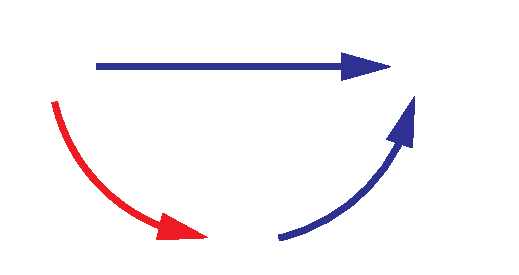
\includegraphics{Figures/Chapter1/decay_CMYK.pdf}%
\end{picture}%
\setlength{\unitlength}{4144sp}%
%
\begingroup\makeatletter\ifx\SetFigFont\undefined%
\gdef\SetFigFont#1#2#3#4#5{%
  \reset@font\fontsize{#1}{#2pt}%
  \fontfamily{#3}\fontseries{#4}\fontshape{#5}%
  \selectfont}%
\fi\endgroup%
\begin{picture}(3939,2094)(2644,-2188)
\put(3286,-736){\makebox(0,0)[rb]{\smash{{\SetFigFont{25}{30.0}{\sfdefault}{\mddefault}{\updefault}{\color[rgb]{0,0,0}$\Bs$}%
}}}}
\put(5761,-736){\makebox(0,0)[lb]{\smash{{\SetFigFont{25}{30.0}{\sfdefault}{\mddefault}{\updefault}{\color[rgb]{0,0,0}$\ffig$}%
}}}}
\put(4501,-421){\makebox(0,0)[b]{\smash{{\SetFigFont{25}{30.0}{\sfdefault}{\mddefault}{\updefault}{\color[rgb]{0,0,1}}%
}}}}
\put(5581,-1771){\makebox(0,0)[lb]{\smash{{\SetFigFont{25}{30.0}{\sfdefault}{\mddefault}{\updefault}{\color[rgb]{0,0,1}}%
}}}}
\put(3331,-1771){\makebox(0,0)[rb]{\smash{{\SetFigFont{25}{30.0}{\sfdefault}{\mddefault}{\updefault}{\color[rgb]{1,0,0}}%
}}}}
\put(4501,-2041){\makebox(0,0)[b]{\smash{{\SetFigFont{25}{30.0}{\sfdefault}{\mddefault}{\updefault}{\color[rgb]{0,0,0}$\Bsb$}%
}}}}
\end{picture}%
}
  \caption{The two interfering decay paths leading to the same final state.}
  \label{app_interference}
\end{figure}

The parameter quantifing \CP violation in the \BsJpsiPhi decay is the so called weak phase \phis.
The Standard Model prediction of the latter parameter as well as its most precice measurement by
\lhcb is:

\noindent The goal of measuring \phis is to look for New Physics effects that Standard Model
does not predict. Given the measuremnt of \equref{app_phis_lhcb} it follwos that \phis is comaptible with
the prediction and any New Physics effects that might apear in \phis must be small.
However, from an experimental point of view the situation is just now becoming intrasting
since the statistical uncertainty of the experimental measuremnt is approaching the Standard
Model prediction. Thus, with the upgraded \lhcb detector the \phis measuremnt is taken to
a high precision era of measurements. Where, along with other observables will most likely
be able to point towards a prticular New Physics model.

\begin{subequations}
  \label{app_phis_lhcb_theo}
  \begin{align}
  \centering
  \phiS{\lhcb}           &=  -0.010 \pm 0.039(\text{total})  \;\; \text{rad},
  \label{app_phis_lhcb}\\
  \phiS{SM,tree}  &= -0.03761 {}^{+0.00073}_{-0.00082}  \;\; \text{rad}.
  \label{app_phis_theo}
\end{align}
\end{subequations}


Entering this promising high precision era comes along with an important consideration that
has to be taken into acount in order to make a robust claim about the presence of New Physics
in \phis. In particular there are certain subleading Standard Model effects that contribute to
the predicted \phis value. These effects become crucial given that fact that, as implied by \equref{app_phis_lhcb_theo},
potential New Physics in \phis are also small. The situation is depicted in the following equation:

\noindent Where delta phis is blah and blah and tree is and peng is.
Thus if contributions from penguin topologies are not properly taken into account there it is
absolutely not posible to distiguish Standard Model diviations from subleading penguin effects.
In order to address another decay invoked in order to be able to estimate penguin contributions
to \phis.

\begin{itemize}
  \item The \BsJpsiKst decay as a probe for penguins
\end{itemize}

\subsubsection{The \lhcb Detector}

\begin{itemize}
\item \lhc cern most powerfull accelrator
\item \lhcb dedicated bfys experiment, unique capabilities, high signal purity. maybe mention proximity to beam and pid.
\item future increase of low pt muon efficiency extents NP reach.
\end{itemize}

\subsubsection{Analysing Particle Collisions}

\begin{itemize}
\item Non infinite resolution and experimental effects and background forces statistical approach.
\item Angular analysis of the decay products to probe polarization fractions. The amplitude has many
      components depending on the oriantation of the spin vectors.
\end{itemize}

\subsubsection{Impact and conclusion}

\begin{itemize}
\item Accordin to Robert recepie Delta phis is found to be blah.
\item This is summarised in the picture blah.
\item It is intreasting becaus blahhhh...
\end{itemize}
